%\documentclass[12pt,preprint]{aastex6}
\documentclass[12pt]{article}

\bibliographystyle{aasjournal}

\usepackage{aas_macros} % need this because not using aastex or emulateapj
\usepackage{graphicx}
\usepackage[suffix=]{epstopdf}
\usepackage{natbib}
\usepackage{amsmath}
%\usepackage{url}
\usepackage{xspace}
\usepackage{fullpage}

%    Make Scientific Notation
\providecommand{\e}[1]{\ensuremath{\times 10^{#1}}}

% make the word Kepler italicized
\newcommand{\Kepler}{\textsl{Kepler}\xspace}

\begin{document}
%%%%%%%%%%%%%%%%%%%%%%


\title{Scientific/Technical/Management}
%Measuring Stellar Rotation with K2
\date{}

\maketitle

%\vspace{-0.5in}
\noindent
We are going to propose for this amazing science...





%%%%%%%%%%%%%%%%%%%
\section{Introduction}


%%%%%%%%%%%%%%%%%%%
\section{Project Description}

%%%%%%%%%
\subsection{Mining K2 Data for Rotation Periods}

%%%%%%%%%
\subsection{Solving the Period Bimodality Mystery}

\begin{figure}[!th]
\centering
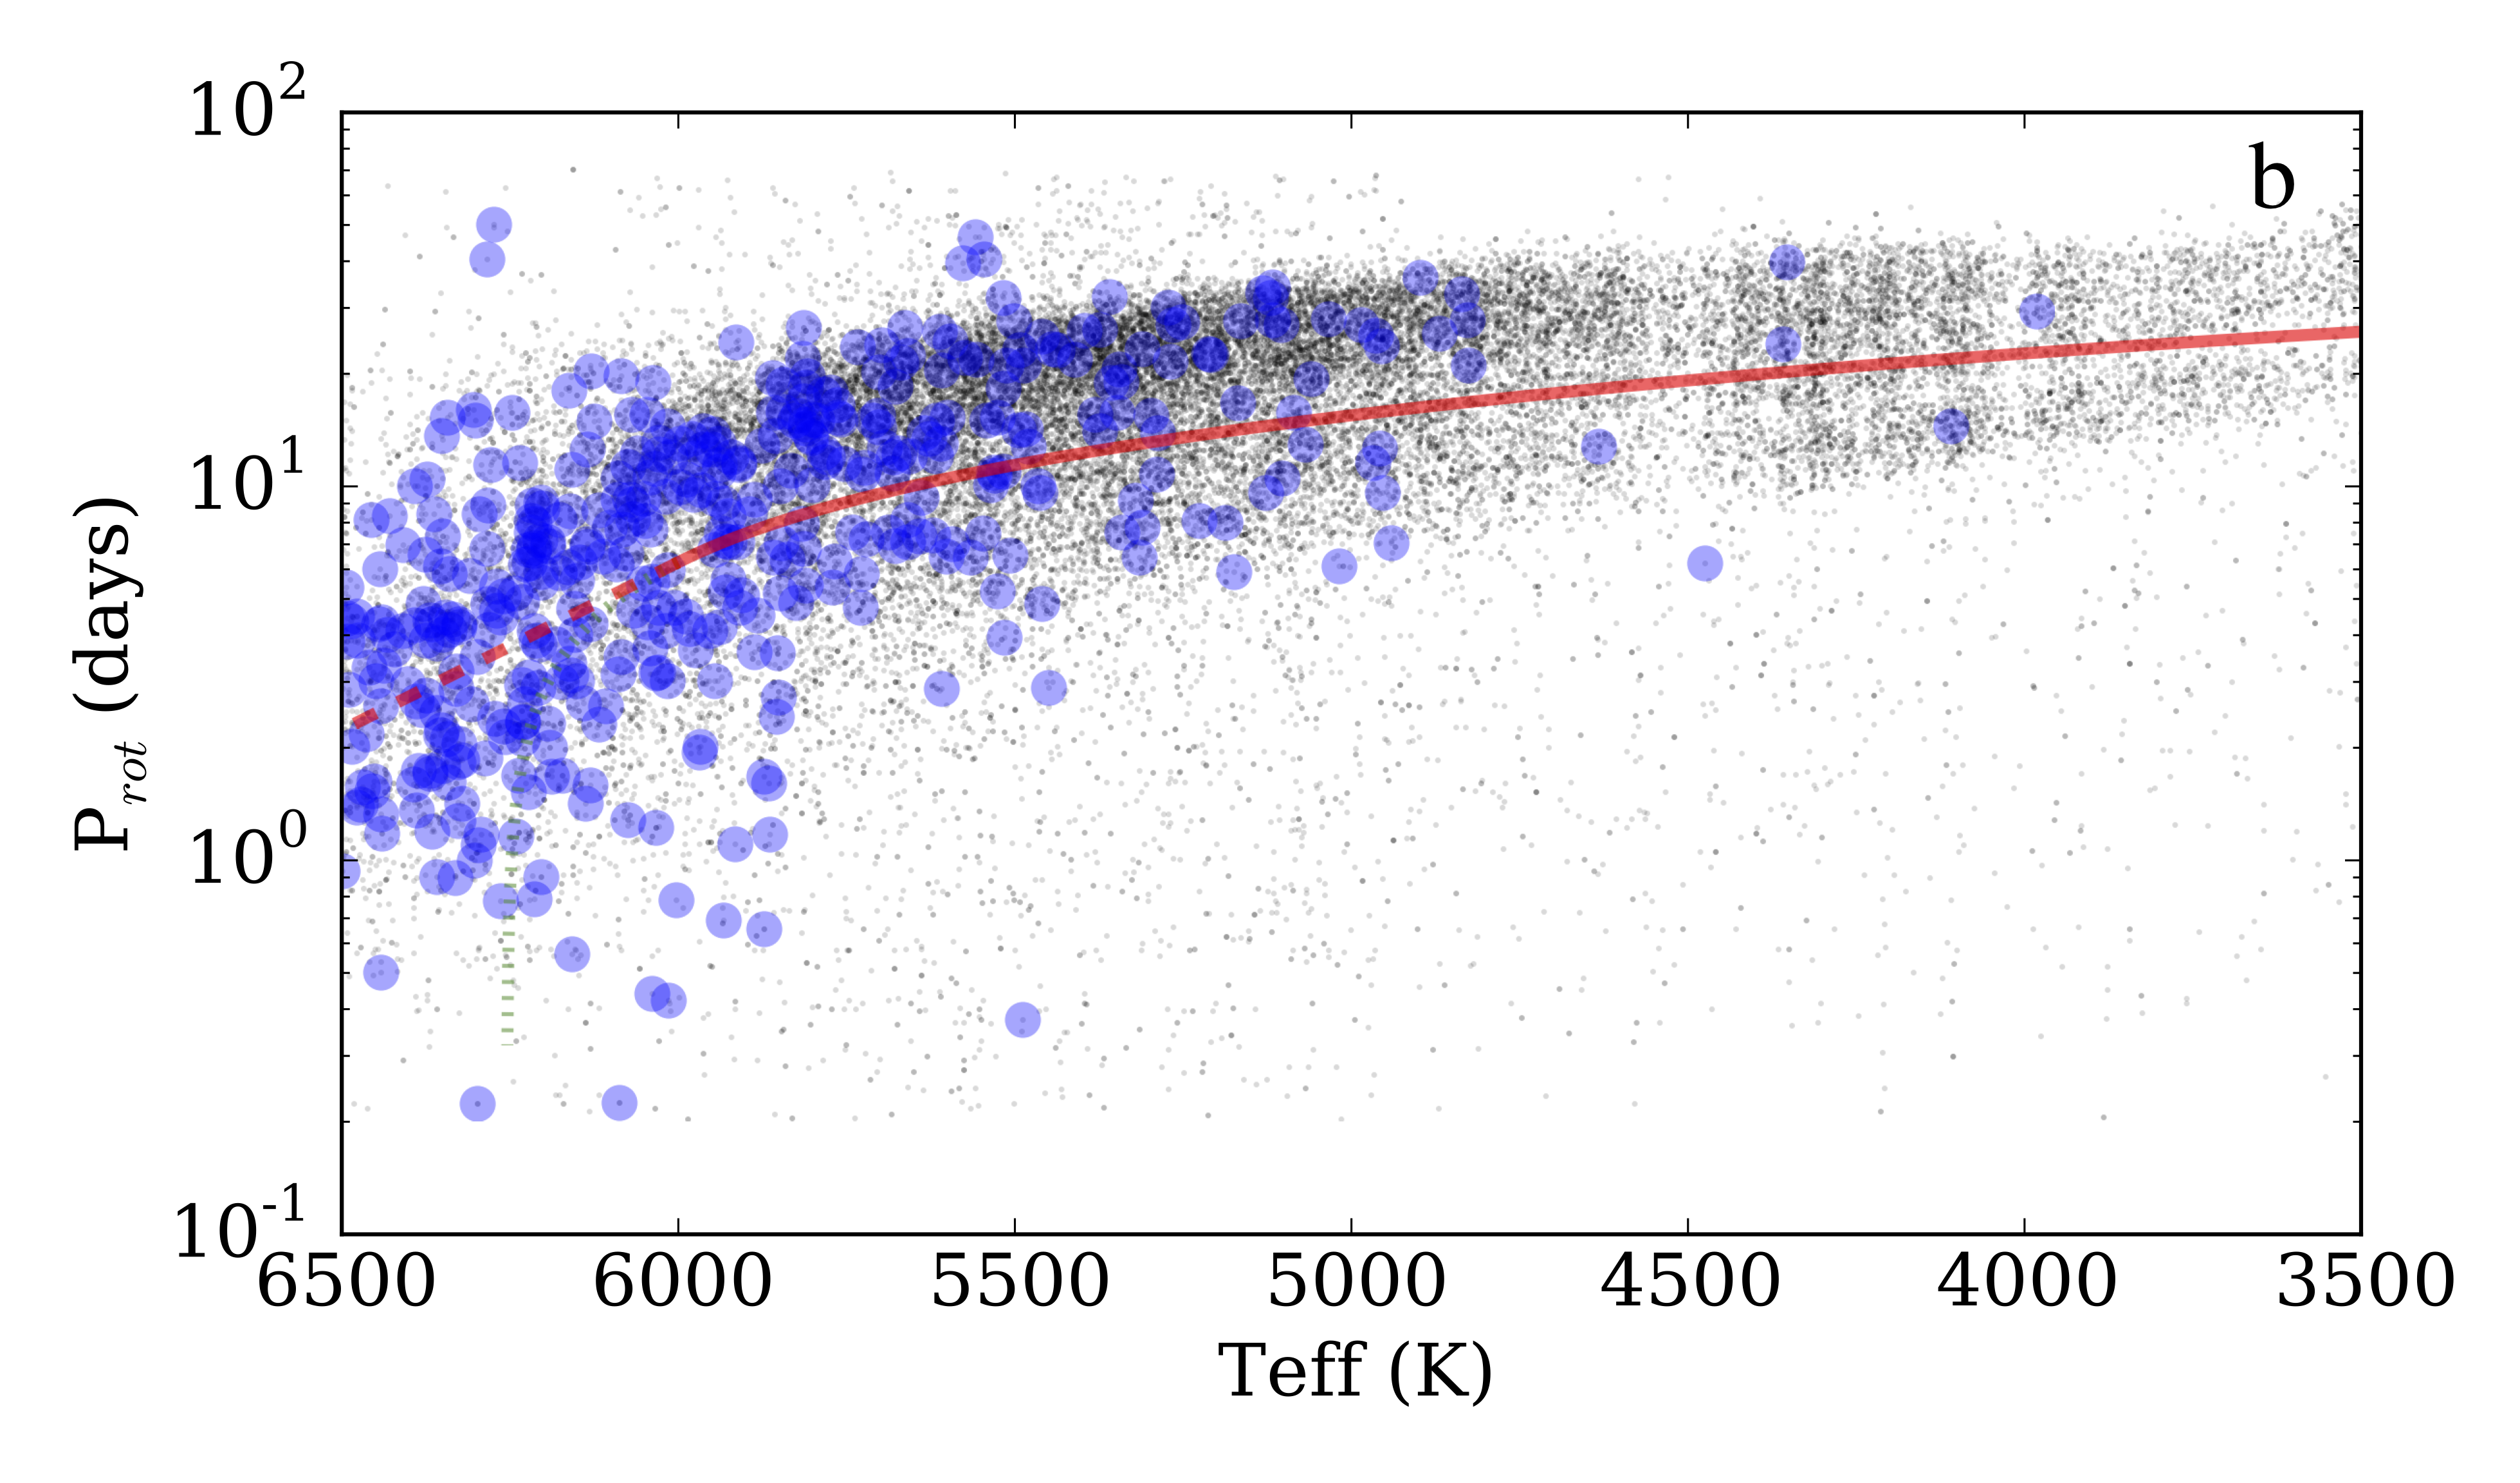
\includegraphics[width=5in]{davenport2016_fig3}
\caption{figure 3 from \citet{davenport2017}, showing bimodality in rotation periods from \Kepler}
\label{fig:bimodal}
\end{figure}




\begin{figure}[!th]
\centering
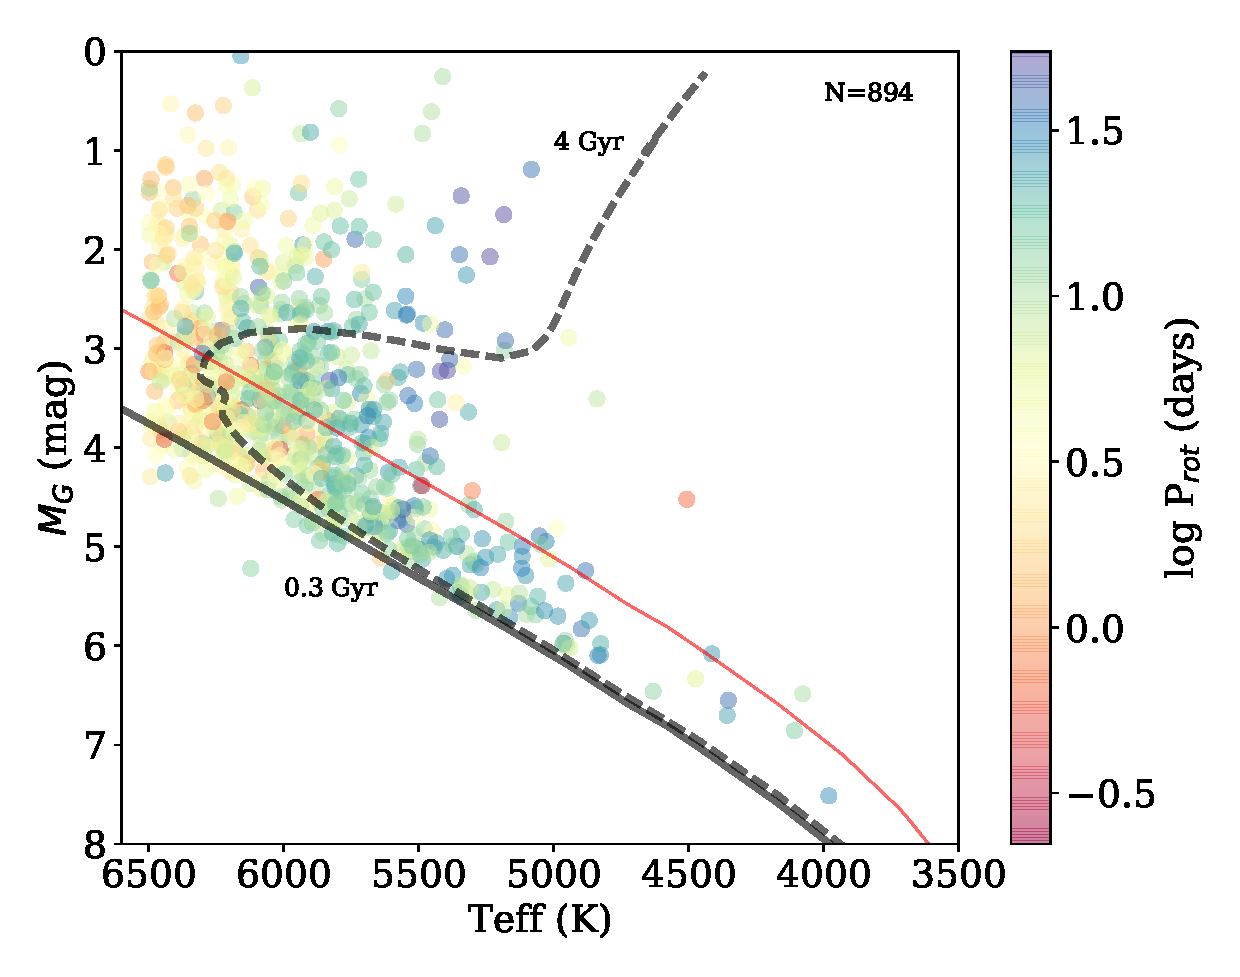
\includegraphics[width=5in]{davenport2016_fig2}
\caption{figure 2 from \citet{davenport2017}, showing temperature from KIC versus absolute magnitude from Gaia}
\label{fig:cmd}
\end{figure}


%%%%%%%%%
\subsection{Age-Dating with K2}

%%%%%%%%%%%%%%%%%%%
\section{Plan of Work}

%%%%%%%%%
\subsection{Measuring Rotation Using TOOL}

%%%%%%%%%
\subsection{Mapping Ages in each Field}

%%%%%%%%%
\subsection{Combining with Gaia}


%%%%%%%%%%%%%%%%%%%
\section{Team Qualifications}


%%%%%%%%%%%%%%%%%%%
%\clearpage
%\pagestyle{empty}

\bibliography{/Users/james/Dropbox/references}


\end{document}

